\documentclass[10pt]{article}
\usepackage{graphicx}
\usepackage{amssymb}
\usepackage[fleqn]{amsmath}
\usepackage{nccmath}
\usepackage{cases}
\usepackage{hyperref}
\usepackage{multicol}
\usepackage{tikz}
\usepackage{pgfplots}
\usepackage{enumitem}
\pgfplotsset{compat=1.18}
\usepackage{float}
\usepackage{pdfpages}

\title{\bf Math 116: Problem Set 3}
\date{1/29/2024}
\author{\bf Owen Jones}
\begin{document}
\maketitle
\begin{enumerate}[label= \arabic*.]
    \item \begin{enumerate}
        \item There exist integers $x,y$ s.t $17x+101y=\gcd(101,17)$\\
        $101=5\cdot 17+16\\
        17=1\cdot 16+1\\
        16=16\cdot 1\\
        \Rightarrow 6\cdot 17-1\cdot 101=1$
        \item $6\cdot 17\equiv 1\pmod {101}\Rightarrow 6={17}^{-1}\pmod {101}$
    \end{enumerate}
    \item \begin{enumerate}
        \item $30=4\cdot 7+2\\
        7=3\cdot2+1\\
        2=2\cdot1\\
        \Rightarrow 13\cdot 7-3\cdot 30=1\\
        \Rightarrow 7d\equiv 1\pmod{30}$ for $d=13$.
        \item We want $D(E(m))=m^{7\cdot d}\equiv m\pmod{31}$.
        By Fermat's Little Theorem, $m^{31}\equiv m\pmod{31}$ $\forall m\in\mathbb{F}_{31}$.
        Let $D(m)=m^{24}\pmod{31}$.
    \end{enumerate} 
    \item \begin{enumerate}
        \item $12x+236y=28$ which is reducible to $3x+59y=7$\\
        $59=19\cdot 3+2\\
        3=1\cdot 2+1\\
        \Rightarrow 20\cdot 3-59=1\Rightarrow 140\cdot3-7\cdot 59=7\\
        140\equiv 22\pmod{59}\\
        x=22+59k$ gives all possible integer solutions.
        \item There are no solutions because $12x,236$ are both divisible by $4$, so $\forall x$ $4$ divides $12x\pmod{236}$. However, $4$ does not divide $30$.
    \end{enumerate}
    \item \begin{enumerate}
        \item $30030=116\cdot 257+218\\
        257=1\cdot 218+39\\
        218=5\cdot 39+23\\
        39=1\cdot 23+16\\
        23=1\cdot 16+7\\
        16=2\cdot 7+2\\
        7=3\cdot 2+1\\
        2=2\cdot 1\\$
        Thus, $\gcd(30030,257)=1$.
        \item $257$ can be factored as a unique product of primes $\prod p_i$. 
        Because $30030$ and $257$ are coprime, $257$ is not divisible by any of $30030's$ factors.
        Moreover, $257$ is not divisible by any prime up to $13$.
        Consider what happens when we divide $257$ by the next largest prime.
        Observe, $257=15\cdot 17+2$.
        It follows that if we divide $257$ by any prime $17$ or larger, the quotient will be smaller than $17$. 
        Thus, $257$ cannot be written as a product of $2$ or more primes because $257$ is not divisible by any prime less than $17$.
        Hence, $257$ must be prime.
    \end{enumerate}
    \item \begin{enumerate}
        \item $4883-4369=514\\
        4369=8\cdot 514+257\\
        514=2\cdot 257\\
        \Rightarrow \gcd(4883,4369)=257$
    \item $4883=19\cdot 257$ and $4369=17\cdot 257$.
    \end{enumerate}
    \item \begin{enumerate}
        \item If $ab\equiv 0\pmod{p}$ then $p|ab$. 
        Since $p$ is prime, and $p\mid ab$ then either $p\mid a$ or $p\mid b$. 
        Because $p\mid a$ or $p\mid b$ then either $a\equiv 0\pmod{p}$ or $b\equiv 0\pmod{p}$
        \item If $\gcd(n,a)=1$ then there exists integers $s,t$ s.t $sn+at=1$.
        Multiplying both sides by $b$ we obtain $snb+abt=b$.  
        Because $b-abt=snb$, $n\mid b-abt$.
        Thus, $b\equiv abt\pmod{n}$.
        However, we know $n\mid ab\Rightarrow abt\equiv 0\pmod{n}$.
        Hence, we $b\equiv 0\pmod{n}\Rightarrow n|b$.
    \end{enumerate}
    \item Let $p\ge3$ be prime and suppose $x^2\equiv1\pmod{p}$. It follows $p|x^2-1\Rightarrow p| (x-1) (x+1)$ by difference of squares. 
    By $6a$, we obtain $p|x-1$ or $p|x+1$. Hence, either $x\equiv 1\pmod{p}$ or $x\equiv-1\pmod{p}$
    Thus, 
    \item Case 1: $p\mid a$\\
    $a\equiv 0\pmod{p}\Rightarrow a^p\equiv 0^p\pmod{p}\Rightarrow a^p\equiv 0\pmod{p}\Rightarrow a^p\equiv a\pmod{p}$.\\
    Case 2: $p\nmid a$\\
    Let $x,x'\in\mathbb{F}_p$. 
    It follows $\exists y,y'\in\mathbb{F}_p$ s.t $ax\equiv y\pmod{p}$ and $ax'\equiv y'\pmod{p}$.
    If $y=y'$, then $p\mid a(x-x')\Rightarrow p\mid(x-x')\Rightarrow x=x'$.
    Thus, $\{0a,a,2a,\ldots,a(p-1)\}$ is just a permutation of $\mathbb{F}_p$.
    Observe $0a\equiv 0\pmod{p}$.
    It follows by multiplying all the non-zero elements together we obtain $a^{p-1}(p-1)!\equiv (p-1)!\pmod{p}$.
    Because $p$ and $(p-1)!$ are relatively prime, $(p-1)!$ has a multiplicative inverse, so $a^{p-1}=1\pmod{p}\Rightarrow a^p\equiv a\pmod{p}$.\\
    \item By Fermat's Little Theorem, $2^{100}\equiv 1\pmod{101}\Rightarrow 2^{10200}\cdot 2^3\equiv 2^3\pmod{101}$. 
    Thus, $2^{10203}\equiv 8\pmod{101}$
    \item $7958357$
    \item \begin{enumerate}
        \item $x=142032116757,y=-466560018663026$
        \item $313608160045*563608596325677\equiv 1\pmod{1030168614988703}$
        \item $343390387426778*313608160045+9620549844273\equiv 2228097317981\pmod{1030168614988703}\\
        \Rightarrow x=313608160045$
    \end{enumerate}
\end{enumerate}
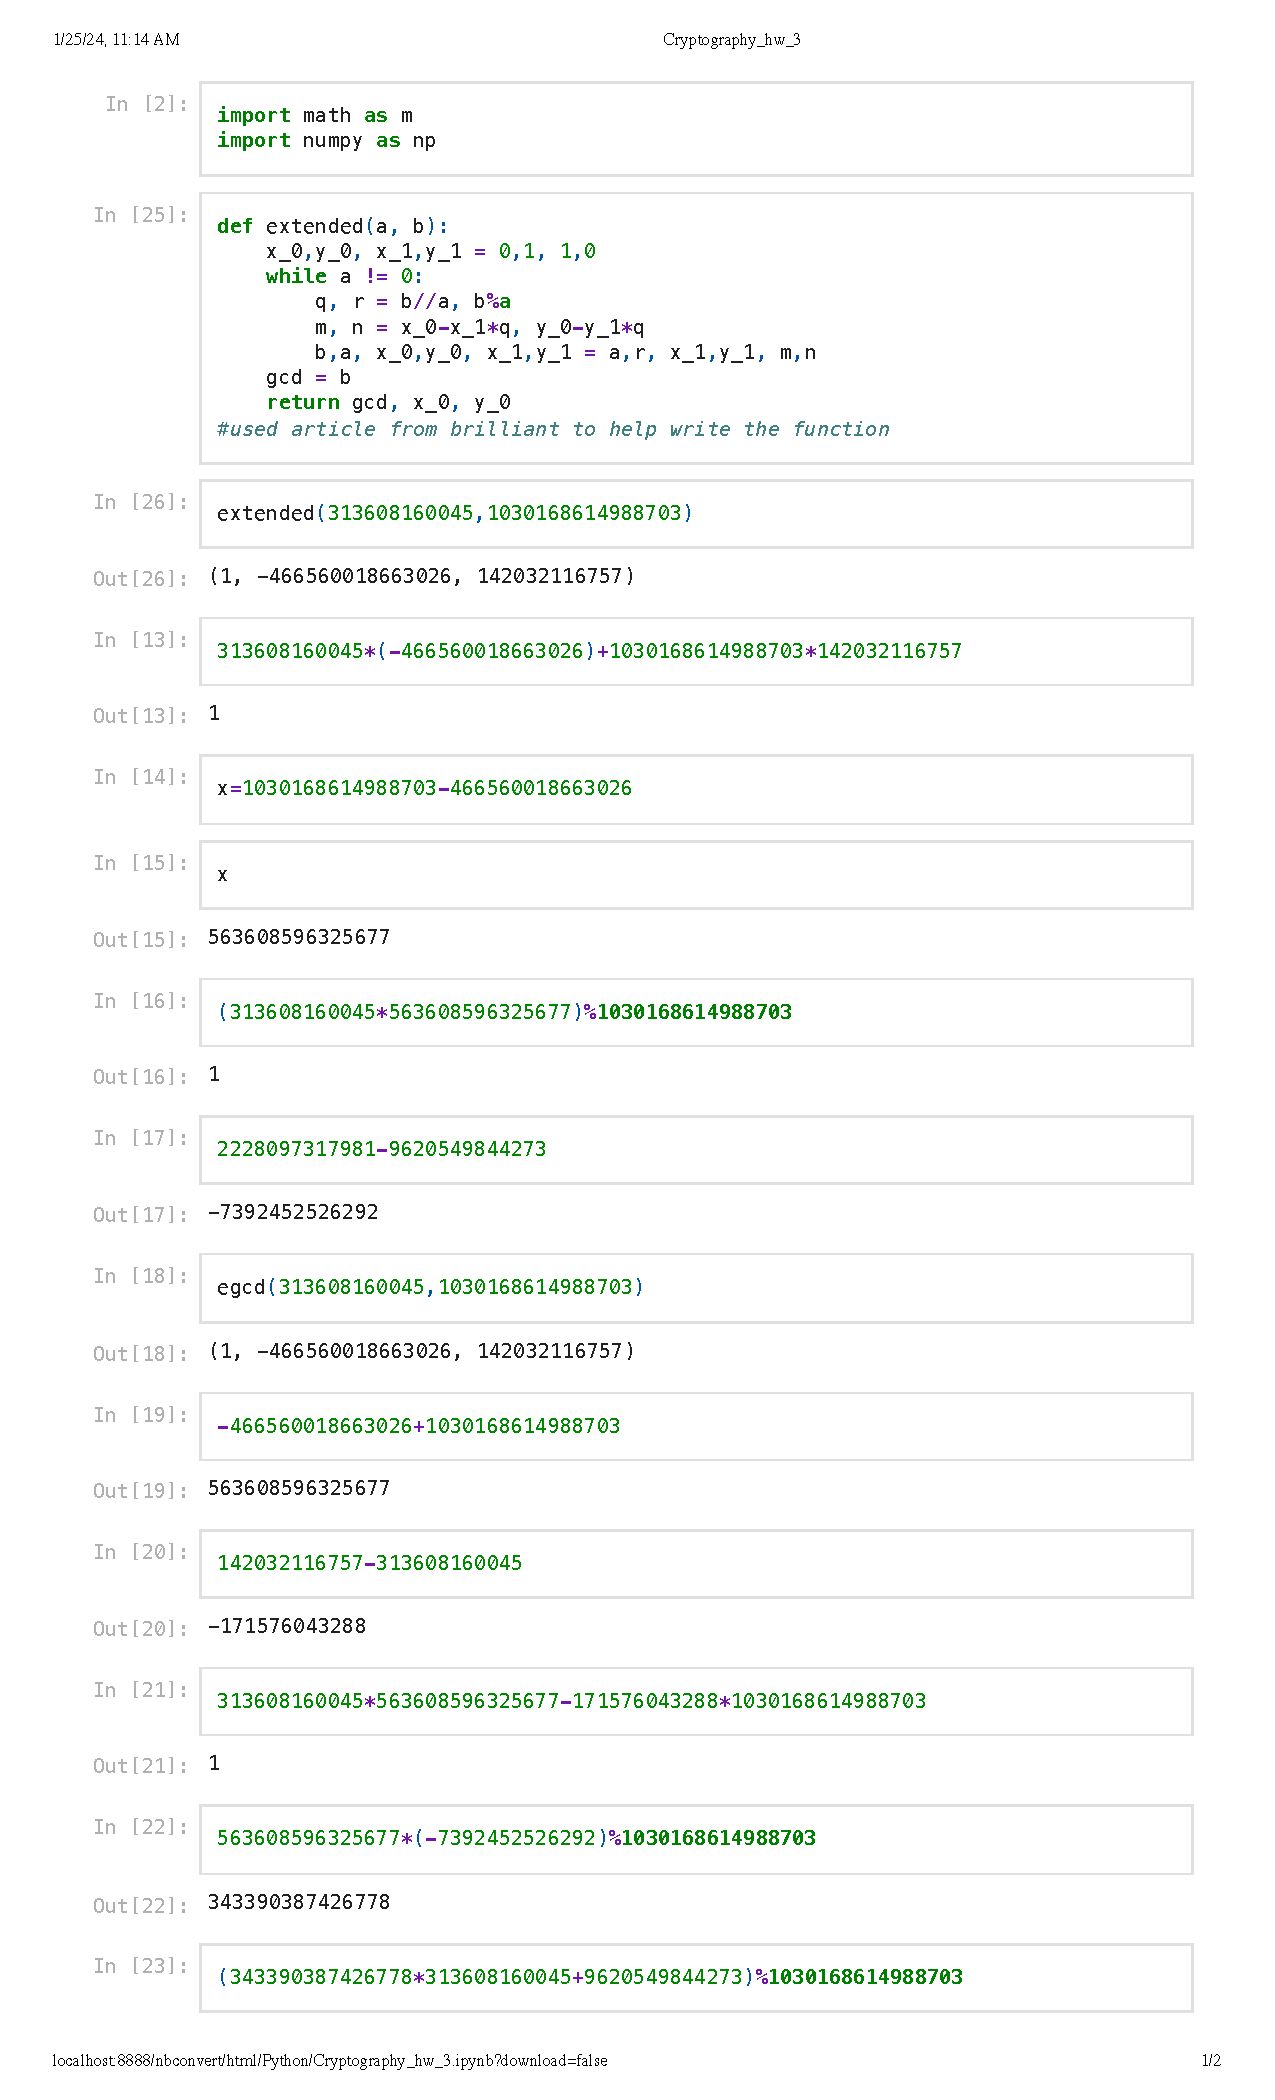
\includepdf[pages=-]{Cryptography_hw_3.pdf}
\end{document}